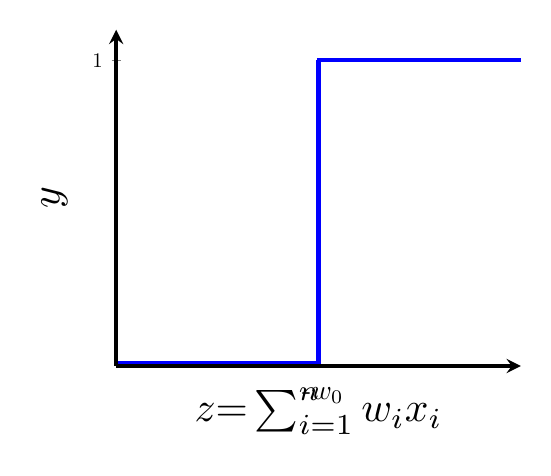
\begin{tikzpicture}[scale=0.75]
	\begin{axis}[
			xmin=-2.5, xmax=2.5,
			ymin=-0.0, ymax=1.1,
			axis lines=left,
			xtick=\empty, ytick={1},
			axis on top=true,
			line width = 2pt,
			%domain=-2.5:2.5,
			ylabel=$y$,
			xlabel=$z{=}\sum_{i=1}^{n} w_i x_i$,
			label style={scale=2}
		]

		\addplot[line width = 5pt, domain=-2.5:0,blue] {0};
		\addplot[line width = 2pt, domain=-0.02:2.5,blue] {1};

		\draw[line width=2pt, blue] (axis cs:0,0) -- (axis cs:0,1);
		%% Add the asymptotes
	\end{axis}

	\node at (3.5,-0.5) {-$w_0$};
\end{tikzpicture}